\documentclass[tikz,border=2pt]{standalone}
\usepackage{pgfplots}
\pgfplotsset{compat=1.18}
\definecolor{raisedgreen}{HTML}{1A7F37}
\begin{document}
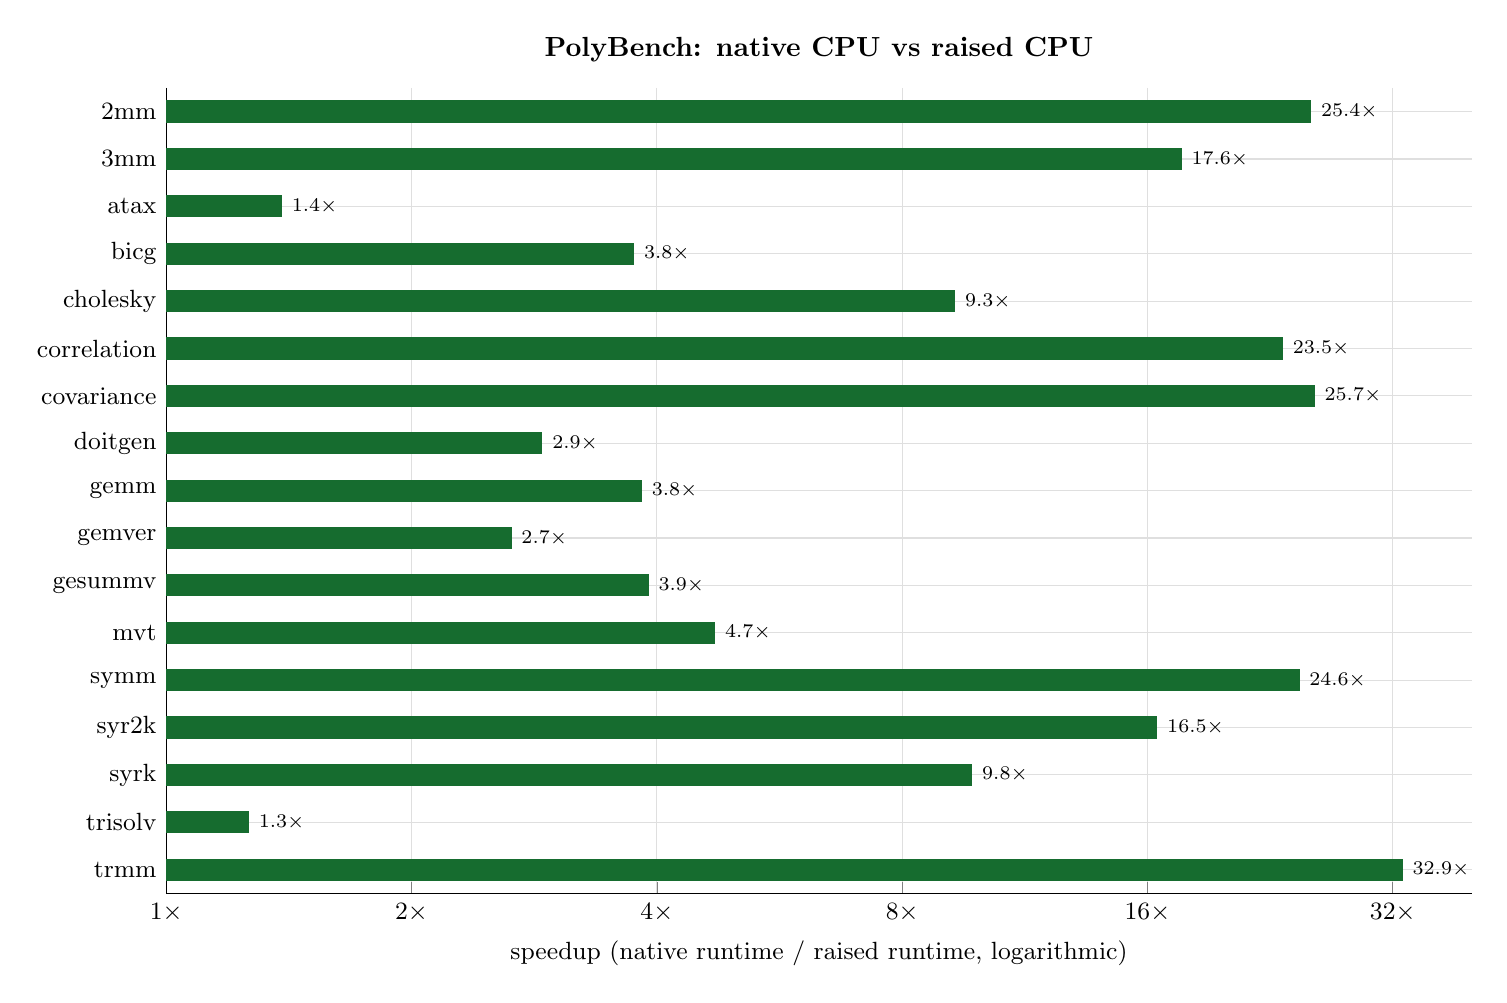
\begin{tikzpicture}
\begin{axis}[
  width=7.15in, height=4.65in,
  title={PolyBench: native CPU vs raised CPU},
  title style={font=\bfseries\normalsize},
  xmode=log, log basis x=2, xmin=1, xmax=40,
  xtick={1,2,4,8,16,32},
  xticklabels={1$\times$,2$\times$,4$\times$,8$\times$,16$\times$,32$\times$},
  xlabel={speedup (native runtime / raised runtime, logarithmic)},
  ymin=-0.5, ymax=16.5,
  ytick={0,1,2,3,4,5,6,7,8,9,10,11,12,13,14,15,16},
  yticklabels={{2mm},{3mm},{atax},{bicg},{cholesky},{correlation},{covariance},{doitgen},{gemm},{gemver},{gesummv},{mvt},{symm},{syr2k},{syrk},{trisolv},{trmm}}, y dir=reverse,
  yticklabel style={font=\small}, xticklabel style={font=\small},
  label style={font=\small}, grid=major,
  major grid style={draw=gray!25}, axis lines*=left,
  clip=false,
]
\draw[draw=raisedgreen!85!black,line width=8pt] (axis cs:1,0) -- (axis cs:25.425029074,0);
\draw[draw=raisedgreen!85!black,line width=8pt] (axis cs:1,1) -- (axis cs:17.634092297,1);
\draw[draw=raisedgreen!85!black,line width=8pt] (axis cs:1,2) -- (axis cs:1.387114172,2);
\draw[draw=raisedgreen!85!black,line width=8pt] (axis cs:1,3) -- (axis cs:3.753077959,3);
\draw[draw=raisedgreen!85!black,line width=8pt] (axis cs:1,4) -- (axis cs:9.298887752,4);
\draw[draw=raisedgreen!85!black,line width=8pt] (axis cs:1,5) -- (axis cs:23.475231954,5);
\draw[draw=raisedgreen!85!black,line width=8pt] (axis cs:1,6) -- (axis cs:25.681532071,6);
\draw[draw=raisedgreen!85!black,line width=8pt] (axis cs:1,7) -- (axis cs:2.895505705,7);
\draw[draw=raisedgreen!85!black,line width=8pt] (axis cs:1,8) -- (axis cs:3.836522779,8);
\draw[draw=raisedgreen!85!black,line width=8pt] (axis cs:1,9) -- (axis cs:2.654216309,9);
\draw[draw=raisedgreen!85!black,line width=8pt] (axis cs:1,10) -- (axis cs:3.910187112,10);
\draw[draw=raisedgreen!85!black,line width=8pt] (axis cs:1,11) -- (axis cs:4.720113059,11);
\draw[draw=raisedgreen!85!black,line width=8pt] (axis cs:1,12) -- (axis cs:24.595063853,12);
\draw[draw=raisedgreen!85!black,line width=8pt] (axis cs:1,13) -- (axis cs:16.459822934,13);
\draw[draw=raisedgreen!85!black,line width=8pt] (axis cs:1,14) -- (axis cs:9.757857573,14);
\draw[draw=raisedgreen!85!black,line width=8pt] (axis cs:1,15) -- (axis cs:1.263697199,15);
\draw[draw=raisedgreen!85!black,line width=8pt] (axis cs:1,16) -- (axis cs:32.932237720,16);
\node[anchor=west,font=\scriptsize] at (axis cs:25.425029074,0) {25.4$\times$};
\node[anchor=west,font=\scriptsize] at (axis cs:17.634092297,1) {17.6$\times$};
\node[anchor=west,font=\scriptsize] at (axis cs:1.387114172,2) {1.4$\times$};
\node[anchor=west,font=\scriptsize] at (axis cs:3.753077959,3) {3.8$\times$};
\node[anchor=west,font=\scriptsize] at (axis cs:9.298887752,4) {9.3$\times$};
\node[anchor=west,font=\scriptsize] at (axis cs:23.475231954,5) {23.5$\times$};
\node[anchor=west,font=\scriptsize] at (axis cs:25.681532071,6) {25.7$\times$};
\node[anchor=west,font=\scriptsize] at (axis cs:2.895505705,7) {2.9$\times$};
\node[anchor=west,font=\scriptsize] at (axis cs:3.836522779,8) {3.8$\times$};
\node[anchor=west,font=\scriptsize] at (axis cs:2.654216309,9) {2.7$\times$};
\node[anchor=west,font=\scriptsize] at (axis cs:3.910187112,10) {3.9$\times$};
\node[anchor=west,font=\scriptsize] at (axis cs:4.720113059,11) {4.7$\times$};
\node[anchor=west,font=\scriptsize] at (axis cs:24.595063853,12) {24.6$\times$};
\node[anchor=west,font=\scriptsize] at (axis cs:16.459822934,13) {16.5$\times$};
\node[anchor=west,font=\scriptsize] at (axis cs:9.757857573,14) {9.8$\times$};
\node[anchor=west,font=\scriptsize] at (axis cs:1.263697199,15) {1.3$\times$};
\node[anchor=west,font=\scriptsize] at (axis cs:32.932237720,16) {32.9$\times$};
\end{axis}
\end{tikzpicture}
\end{document}
